\documentclass[11pt]{article}
\input{/Users/markwang/.preamble}
\begin{document}



\textbf{Question 1 Regularized linear regression.}

For some $\lambda > 0$, we have 
\[
    \mathcal{E}_{reg} = 
    \frac{1}{2N} \sum_{i=1}^N (y^{(i)} - t^{(i)})^2 + \frac{\lambda}{2} \sum_{j=1}^D w_j^2    
\]

\begin{enumerate}
    \item Determine the gradient descent update rules for the regularized cost function $\mathcal{E}_{reg}$.\\
    Derive the partial of cost function
    \[
        \frac{\partial \mathcal{E}_{reg}}{\partial w_j}
        = 
        \frac{1}{N} \sum_{i=1}^N x_j^{(i)} (y^{(i)} - t^{(i)}) + \lambda w_j
    \]
    Therefore 
    \begin{align*}
        w_j &\leftarrow w_j - \alpha \frac{\partial\mathcal{E}_{reg}}{\partial w_j} = \alpha \left(
            \frac{1}{N} \sum_{i=1}^N x_j^{(i)} (y^{(i)} - t^{(i)}) + \lambda w_j 
        \right) \\
        b &\leftarrow b - \alpha \frac{\partial\mathcal{E}_{reg}}{\partial b}  = \alpha \left(
            \frac{1}{N} \sum_{i=1}^N (y^{(i)} - t^{(i)}) + \lambda b
        \right)
    \end{align*}
    \item It’s also possible to solve the regularized regression problem directly by setting the partial derivatives equal to zero. In this part, for simplicity, we will drop the bias term from the model, so our model is:
    \[
        y = \sum_{j=1}^D w_j x_j    
    \]
    Now derive partials of $\mathcal{E}_{reg}$ as a system of linear equations. By setting $\frac{\partial \mathcal{E}_{reg}}{\partial w_j} = 0$ we have
    \begin{align*}
        \frac{1}{N}  \sum_{j'=1}^D (  \sum_{i=1}^N x_j^{(i)} x_{j'}^{(i)}) w_{j'} - \frac{1}{N} \sum_{i=1}^N x_j^{(i)} t^{(i)} + \lambda w_j
        &= 0 \\ 
        \sum_{j'=1}^D ( \frac{1}{N} \sum_{i=1}^N x_j^{(i)} x_{j'}^{(i)} + \lambda \mathbbm{1}_{j'=j}) w_{j'} - \frac{1}{N} \sum_{i=1}^N x_j^{(i)} t^{(i)} 
        &= 0 \\
        \sum_{j'=1}^D A_{jj'} w_{j'} &= c_j \\ 
    \end{align*}
    where 
    \[
        A_{jj'} =  \frac{1}{N}\sum_{i=1}^N x_j^{(i)} x_{j'}^{(i)} + \lambda \mathbbm{1}_{j'=j}
        \quad \quad \quad \quad 
        c_j = \frac{1}{N} \sum_{i=1}^N x_j^{(i)} t^{(i)}
    \]
    or vectorized form 
    \[
        \matr{A} = \frac{1}{N} \matr{X^TX} + \lambda \matr{I} 
        \quad \quad \quad \quad 
        \matr{c} = \frac{1}{N} \matr{X^T t}   
    \]
\end{enumerate}



\textbf{Question 2 Visualizing the cost function.}


\begin{enumerate}
    \item Write the cost in the form 
    \[
        \mathcal{E} = c_1 (w_1 - d_1)^2 + c_2 (w_2- d_2)^2 + \mathcal{E}_0    
    \]
    Simply substitute value in to the formula of the cost function $\mathcal{E}$
    \begin{align*}
        \mathcal{E}
        = \frac{1}{2N} ||\matr{ Xw - t} ||^2
        &= \frac{1}{6} 
        \left|\left| 
        \begin{pmatrix}
            2 & 0 \\
            0 & 1 \\ 
            0 & 1 \\ 
        \end{pmatrix} 
        \begin{pmatrix}
            w_1 \\ w_2
        \end{pmatrix}
        -
        \begin{pmatrix} 
            1 \\ 2 \\ 0 \\
        \end{pmatrix} 
        \right|\right|^2 \\ 
        &= 
        \frac{1}{6} \left(
            (2w_1 - 1)^2 + (w_2 - 2)^2 + w_2^2
        \right) \\
        &= \frac{2}{3}(w_1 - \frac{1}{2})^2 + \frac{1}{3} (w_2 - 1)^2 + \frac{1}{3}
    \end{align*}
    \item Since $c_1, c_2 > 0$, this corresponds to an axis-aligned ellipse. Sketch the ellipse by hand for $\mathcal{E} = 1$. Label the center and radii of the ellipse. \\
    \[
        \mathcal{E} = 1 \quad \quad \implies \quad \quad 
        (w_1 - \frac{1}{2})^2 + \frac{1}{2} (w_2 - 1)^2 = 1
    \]
    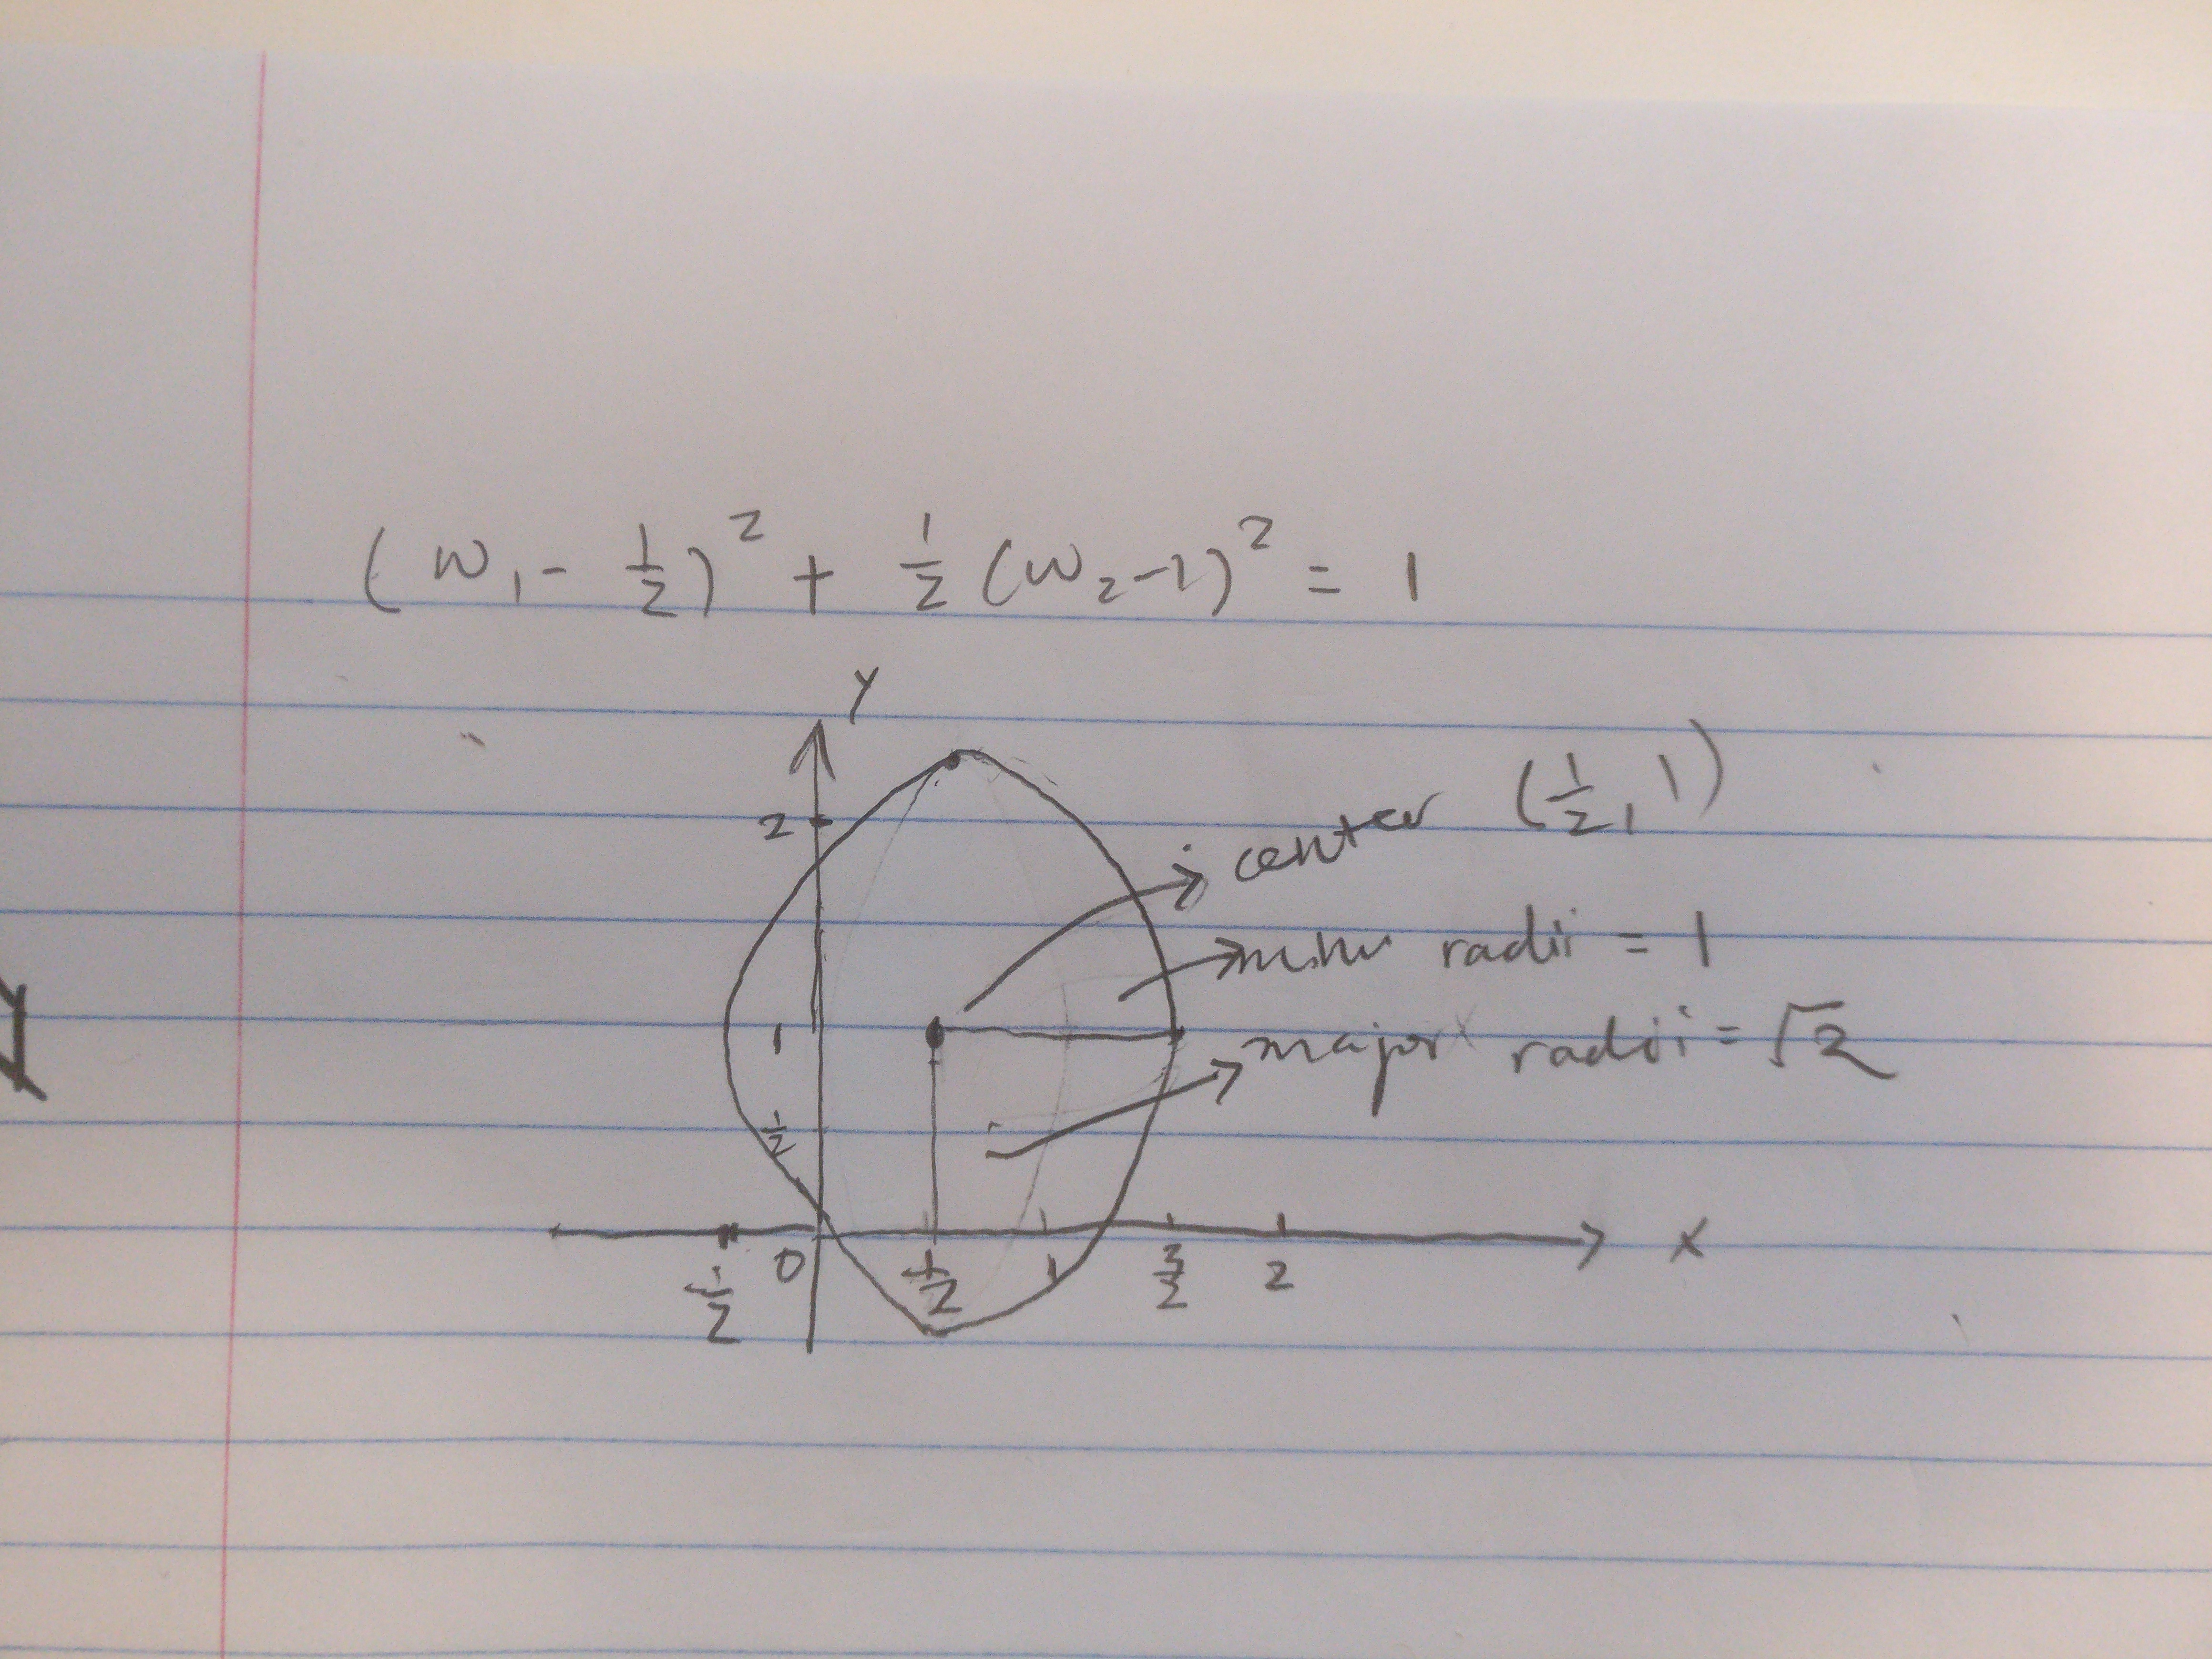
\includegraphics[width=\textwidth]{ellipse.jpg}
\end{enumerate}


\end{document}
